\section{最优解的判别}
\label{sec:moo-optimality}

标量化回答的是“给定偏好求一个解”。这一节换一个问法：手里已经有一个候选点，只看它附近的导数信息，能否判断它值不值得继续改进？

单目标问题中，这个问题由“存在下降方向”来回答。多目标问题中对应的问题是：是否存在一个可行的小步，使所有目标都下降？本节先在无约束内点回答，再加上约束。全节都要把两种结论分开：不存在共同下降方向是一个局部的必要条件，它要成为全局Pareto最优的证据，还需要凸性和权重条件。

\subsection{共同下降方向}
\label{sec:moo-common-descent}

设$\bm{x}$是$\bm{C}$的内点，各$f_i$在$\bm{x}$处可微，记
\[
 \bm{g}_i=\nabla f_i(\bm{x}),\qquad i=1,\ldots,m.
\]
我们想知道，从$\bm{x}$出发能不能让全部目标一起变小。

\paragraph{方向的定义}
一个方向$\bm{d}$若满足
\begin{equation}
 \langle\bm{g}_i,\bm{d}\rangle<0\quad\text{对所有}\ i=1,\ldots,m,
 \label{eq:moo-common-descent}
\end{equation}
就称为\term{共同下降方向}（common descent direction）。由一阶Taylor展开，沿这样的$\bm{d}$走足够小的一步，每个目标都严格下降，当前点就被支配了。

每个不等式要求$\bm{d}$落在以$\bm{g}_i$为法向的一个开半空间内，所有这些半空间的公共部分就是全部共同下降方向。图~\ref{fig:moo-common-descent}(a)中两个梯度夹角小于$180^\circ$，绿色楔形就是这个公共部分。

等高线上的直观是：站在山坡上，每个目标各有一个下山的半平面。几个半平面还有公共的部分，就能一步同时往几座山的下坡方向走。公共部分消失时，不管往哪里走，至少有一个目标的一阶变化不是下降。

\begin{BookInlineFigure}
  \centering
  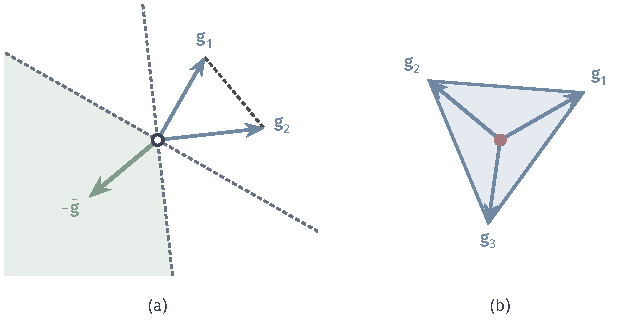
\includegraphics[width=104.8mm]{figures/05-optimization/07-multiple-criteria-and-nested-optimization/tikz/moo-common-descent/figure.pdf}
  \caption{共同下降方向与梯度的凸包，空心点和红点是原点。(a)两个梯度的凸包是虚线线段，不含原点；两条灰色虚线分别垂直于$\bm{g}_1,\bm{g}_2$，绿色楔形是共同下降方向。(b)三个梯度的凸包是浅蓝三角形，原点（红点）在其内部，此时不存在共同下降方向。}
  \label{fig:moo-common-descent}
\end{BookInlineFigure}

\paragraph{用梯度的凸包判别}
图~\ref{fig:moo-common-descent}提示了判别方法。把各梯度当作点，看它们的\term{凸包}（convex hull）
\[
 \operatorname{conv}\{\bm{g}_1,\ldots,\bm{g}_m\}=\Bigl\{\sum_{i=1}^m\theta_i\bm{g}_i:\bm{\theta}\in\Delta_m\Bigr\},
\]
也就是全部梯度的加权平均组成的集合。下面的引理说，这个集合是否包含原点，恰好决定共同下降方向是否存在。

\begin{lemma}[共同下降方向的存在性]
\label{lem:moo-gordan}
存在满足式~\eqref{eq:moo-common-descent}的$\bm{d}$，当且仅当$\bm{0}\notin\operatorname{conv}\{\bm{g}_1,\ldots,\bm{g}_m\}$。
\end{lemma}

\begin{proof}
先设$\bm{0}$在凸包中，即有$\bm{\theta}\in\Delta_m$使$\sum_i\theta_i\bm{g}_i=\bm{0}$。若式~\eqref{eq:moo-common-descent}成立，把它们按$\theta_i\geq0$加权相加，由于至少有一个$\theta_i>0$，得到
\[
 0=\Bigl\langle\sum_i\theta_i\bm{g}_i,\bm{d}\Bigr\rangle=\sum_i\theta_i\langle\bm{g}_i,\bm{d}\rangle<0,
\]
矛盾。

再设$\bm{0}$不在凸包中。凸包是非空紧凸集，记原点在它上面的投影为$\bar{\bm{g}}\neq\bm{0}$。第~\ref{chap:nonsmooth-composite-optimization}章的投影性质给出，对凸包中任一点$\bm{v}$，
\[
 \langle\bm{0}-\bar{\bm{g}},\bm{v}-\bar{\bm{g}}\rangle\leq0.
\]
取$\bm{v}=\bm{g}_i$，整理得
\[
 \langle\bm{g}_i,\bar{\bm{g}}\rangle\geq\lVert\bar{\bm{g}}\rVert_2^2>0.
\]
令$\bm{d}=-\bar{\bm{g}}$，式~\eqref{eq:moo-common-descent}成立。
\end{proof}

第二部分的构造不只是存在性证明，第~\ref{sec:moo-mgda}节就要把它变成算法。原点在凸包中的情形有专门的名称。

\begin{definition}[Pareto驻定]
\label{def:moo-stationary}
若存在$\bm{\theta}\in\Delta_m$，使
\begin{equation}
 \sum_{i=1}^m\theta_i\nabla f_i(\bm{x})=\bm{0},
 \label{eq:moo-stationary}
\end{equation}
称$\bm{x}$为\term{Pareto驻定}（Pareto stationary）点。
\end{definition}

$m=1$时，$\theta_1=1$，式~\eqref{eq:moo-stationary}就是$\nabla f_1=\bm{0}$，回到单目标的驻定点。多目标时，并不要求每个梯度为零，只要求它们能以非负系数相互抵消。

\paragraph{必要性与连续例}
局部最优点不允许共同下降，由此得到一阶必要条件。

\begin{theorem}[Pareto驻定的必要性]
\label{thm:moo-stationary-necessary}
设$\bm{x}$是$\bm{C}$的内点，各$f_i$在$\bm{x}$处可微。若$\bm{x}$是局部弱Pareto最优点，特别地若$\bm{x}$是局部Pareto最优点，则$\bm{x}$是Pareto驻定点。
\end{theorem}

\begin{proof}
若$\bm{x}$不是Pareto驻定点，由引理~\ref{lem:moo-gordan}，存在满足式~\eqref{eq:moo-common-descent}的$\bm{d}$。对充分小的$t>0$，由Taylor展开，
\[
 f_i(\bm{x}+t\bm{d})=f_i(\bm{x})+t\langle\bm{g}_i,\bm{d}\rangle+o(t)<f_i(\bm{x})
\]
对所有$i$成立。$\bm{x}$是内点，$\bm{x}+t\bm{d}$可行，这与局部弱Pareto最优矛盾。
\end{proof}

下面在例~\eqref{eq:moo-iso}上检查，见图~\ref{fig:moo-gradient-points}。此时$\bm{g}_1=\bm{x}-\bm{a}$，$\bm{g}_2=\bm{x}-\bm{b}$。在线段外的点$\bm{p}=(1,1)$处，
\[
 \bm{g}_1=(0,1),\qquad\bm{g}_2=(1,0).
\]
它们的凸组合是$(1-\theta,\theta)$，永远不为零，所以$\bm{p}$不是驻定点。取$\theta=1/2$得最短的组合$(1/2,1/2)$，方向$\bm{d}=(-1/2,-1/2)$使两个目标同时下降。

在线段上的点$\bm{q}=(0.6,0.4)$处，
\[
 \bm{g}_1=(-0.4,0.4),\qquad\bm{g}_2=(0.6,-0.6).
\]
两个梯度方向相反，取$\bm{\theta}=(0.6,0.4)$得到$0.6\bm{g}_1+0.4\bm{g}_2=\bm{0}$，$\bm{q}$是驻定点。这里的$\theta_1=0.6$恰好等于式~\eqref{eq:moo-iso-weighted}中选中$\bm{q}$的权重$w$。

\begin{BookInlineFigure}
  \centering
  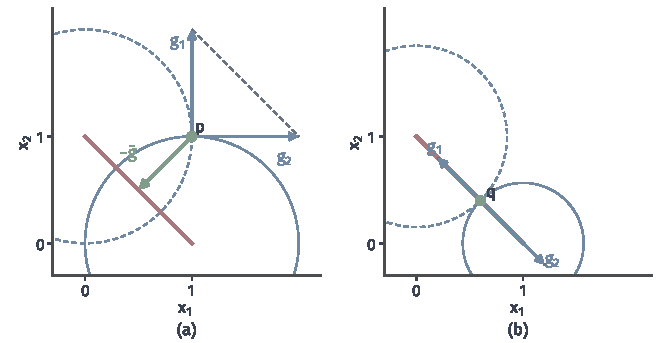
\includegraphics[width=112mm]{figures/05-optimization/07-multiple-criteria-and-nested-optimization/matplotlib/moo-gradient-points/figure.pdf}
  \caption{例~\eqref{eq:moo-iso}中两点处的梯度，圆是经过该点的两条等高线，红色线段是Pareto解集。(a)线段外的点$\bm{p}=(1,1)$，两个梯度的凸包（虚线）不含零，绿色箭头是最小范数组合的反方向。(b)线段上的点$\bm{q}=(0.6,0.4)$，两个梯度反向，凸包含零，两条等高线在$\bm{q}$相切。}
  \label{fig:moo-gradient-points}
\end{BookInlineFigure}

图~\ref{fig:moo-gradient-points}(b)还显示了一件事：在$\bm{q}$处两个圆相切，要进入一个圆的内部，就必须走出另一个圆。这是取舍的局部形象。

\paragraph{驻定点不一定是Pareto最优点}
定理~\ref{thm:moo-stationary-necessary}只有一个方向。Pareto驻定只排除严格的共同下降，并不排除“有的目标不变，另一些目标下降”。取$\bm{x}\in\mathbb{R}^2$，
\begin{equation}
 f_1(\bm{x})=x_1^2,\qquad f_2(\bm{x})=x_2.
 \label{eq:moo-stationary-weak}
\end{equation}
在原点，$\bm{g}_1=\bm{0}$，$\bm{g}_2=(0,1)$，取$\bm{\theta}=(1,0)$，式~\eqref{eq:moo-stationary}成立。可是沿$(0,-t)$移动，$f_1$保持为$0$，$f_2$严格下降，原点被支配，见图~\ref{fig:moo-stationary-gap}(a)。

问题还可能更严重。取一元函数$f_1(x)=f_2(x)=-x^2$，$x=0$是Pareto驻定点，但$x=\pm1$处两个目标都更小，原点连弱Pareto最优点都不是，见图~\ref{fig:moo-stationary-gap}(b)。这与单目标的极大点也是驻定点是同一回事。

\begin{BookInlineFigure}
  \centering
  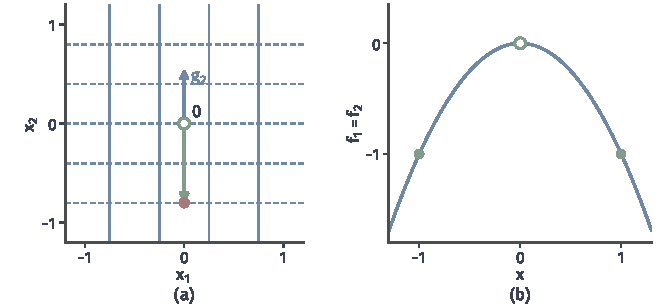
\includegraphics[width=112mm]{figures/05-optimization/07-multiple-criteria-and-nested-optimization/matplotlib/moo-stationary-gap/figure.pdf}
  \caption{Pareto驻定不足以断定最优。(a)式~\eqref{eq:moo-stationary-weak}，竖线是$f_1$的等高线，虚线是$f_2$的等高线；在空心点（原点）处$\bm{g}_1=\bm{0}$，沿绿色箭头$f_1$不变、$f_2$下降，红点支配原点。(b)$f_1=f_2=-x^2$，空心点是驻定点，两个绿点的目标都更小。}
  \label{fig:moo-stationary-gap}
\end{BookInlineFigure}

\paragraph{凸问题中的充分性}
要从驻定走到最优，需要凸性。此时式~\eqref{eq:moo-stationary}的系数$\bm{\theta}$恰好提供了一组权重。

\begin{theorem}[凸问题的驻定点]
\label{thm:moo-stationary-sufficient}
设$\bm{C}=\mathbb{R}^n$，各$f_i$凸且可微，$\bm{x}$满足式~\eqref{eq:moo-stationary}。则$\bm{x}$是$\sum_i\theta_if_i$的全局最小点，因而是全局弱Pareto最优点；若所有$\theta_i>0$，$\bm{x}$是全局Pareto最优点。
\end{theorem}

\begin{proof}
$\sum_i\theta_if_i$是凸函数，其梯度在$\bm{x}$处为零，由第~\ref{chap:optimization}章的一阶条件，$\bm{x}$是它的全局最小点。再由定理~\ref{thm:moo-weighted}得结论。
\end{proof}

式~\eqref{eq:moo-stationary-weak}的原点符合定理的条件，但$\theta_2=0$，所以只能得到弱Pareto最优，这正好和前面看到的现象一致。在例~\eqref{eq:moo-iso}的线段内部，$\bm{\theta}$的两个分量都为正，得到的是Pareto最优。

\subsection{可行方向}
\label{sec:moo-feasible-direction}

候选点若在可行集边界上，只有一部分方向走得动，梯度的凸包不含零也不等于存在可行的共同下降方向。这一小节把判别限制在可行方向上，并调用第~\ref{chap:constrained-optimality}章的约束条件。

\paragraph{问题与记号}
由于$m$已经用来表示目标个数，约束的下标改写为
\[
 \bm{C}=\{\bm{x}:g_j(\bm{x})\leq0,\ j=1,\ldots,q,\ \ h_k(\bm{x})=0,\ k=1,\ldots,p\}.
\]
活动集$A(\bar{\bm{x}})$、切锥$\bm{T}_{\bm{C}}(\bar{\bm{x}})$、线性化锥、LICQ、MFCQ的含义都与第~\ref{chap:constrained-optimality}章相同，只是把不等式的下标换成了$j$，等式的下标换成了$k$。这里的$g_j$是约束函数，加粗的$\bm{g}_i$才是目标的梯度。

\paragraph{切锥上的必要条件}
“能走的方向”由切锥描述，一阶必要条件的形式与单目标的切锥条件相同。

\begin{theorem}[切锥上的必要条件]
\label{thm:moo-tangent-necessary}
设$\bar{\bm{x}}$是局部弱Pareto最优点，各$f_i$在$\bar{\bm{x}}$处可微。则不存在$\bm{d}\in\bm{T}_{\bm{C}}(\bar{\bm{x}})$，使
\begin{equation}
 \langle\nabla f_i(\bar{\bm{x}}),\bm{d}\rangle<0\quad\text{对所有}\ i=1,\ldots,m.
 \label{eq:moo-tangent-descent}
\end{equation}
\end{theorem}

\begin{proof}
设这样的$\bm{d}$存在。由切锥定义，有可行点列$\bm{x}^{(k)}\to\bar{\bm{x}}$与$t_k\downarrow0$，使$(\bm{x}^{(k)}-\bar{\bm{x}})/t_k\to\bm{d}$。Taylor展开并除以$t_k$，
\[
 \frac{f_i(\bm{x}^{(k)})-f_i(\bar{\bm{x}})}{t_k}\to\langle\nabla f_i(\bar{\bm{x}}),\bm{d}\rangle<0.
\]
目标个数有限，所以$k$足够大时，所有$f_i(\bm{x}^{(k)})<f_i(\bar{\bm{x}})$同时成立，与局部弱Pareto最优矛盾。
\end{proof}

\paragraph{目标权重与约束乘子}
切锥不容易计算。约束资格把它换成线性化锥，结论就可以用乘子写出来，形式上是把KKT条件中目标的梯度换成目标梯度的凸组合。

证明不用重新做Farkas那一套，把问题改写成单目标问题即可：引入一个变量$t$代表“所有目标相对当前点的最大变化”，然后要求这个变化不能为负。

\begin{theorem}[多目标KKT必要条件]
\label{thm:moo-kkt-necessary}
设$f_i$、$g_j$、$h_k$在局部弱Pareto最优点$\bar{\bm{x}}$附近连续可微，并且$\bar{\bm{x}}$满足MFCQ。则存在$\bm{\theta}\in\Delta_m$，$\bm{\lambda}\geq\bm{0}$，$\bm{\nu}$，使
\begin{equation}
 \sum_{i=1}^m\theta_i\nabla f_i(\bar{\bm{x}})
 +\sum_{j=1}^q\lambda_j\nabla g_j(\bar{\bm{x}})
 +\sum_{k=1}^p\nu_k\nabla h_k(\bar{\bm{x}})=\bm{0},
 \label{eq:moo-kkt}
\end{equation}
并且$\lambda_jg_j(\bar{\bm{x}})=0$对所有$j$成立。
\end{theorem}

\begin{proof}
考虑变量为$(\bm{x},t)$的单目标问题
\[
 \min_{\bm{x},t}\ t\quad\text{s.t.}\quad
 f_i(\bm{x})-f_i(\bar{\bm{x}})-t\leq0,\ \ \bm{x}\in\bm{C}.
\]

先说明$(\bar{\bm{x}},0)$是它的局部最小点。若$\bm{x}$靠近$\bar{\bm{x}}$，$(\bm{x},t)$可行且$t<0$，则$f_i(\bm{x})<f_i(\bar{\bm{x}})$对所有$i$成立，与局部弱Pareto最优矛盾。

再说明MFCQ在$(\bar{\bm{x}},0)$处成立。设$\bar{\bm{d}}$是原约束的MFCQ方向。增广问题中等式约束的梯度是$(\nabla h_k,0)$，线性无关；取方向$(\bar{\bm{d}},\sigma)$，$\sigma$足够大，则
\[
 \langle\nabla f_i(\bar{\bm{x}}),\bar{\bm{d}}\rangle-\sigma<0\quad\text{对所有}\ i,
\]
其余条件与原约束相同。

由第~\ref{chap:constrained-optimality}章的KKT必要性定理，存在乘子$\bm{\theta}\geq\bm{0}$（对应$f_i-f_i(\bar{\bm{x}})-t\leq0$）、$\bm{\lambda}\geq\bm{0}$与$\bm{\nu}$。对$t$的驻定条件是$1-\sum_i\theta_i=0$，所以$\bm{\theta}\in\Delta_m$；对$\bm{x}$的驻定条件是式~\eqref{eq:moo-kkt}；互补条件来自原约束的互补松弛。
\end{proof}

约束资格不能省。取一元变量，$f_1(x)=f_2(x)=x$，约束$g(x)=x^2\leq0$。可行集只有$\{0\}$，所以$0$是Pareto最优点。但$\nabla f_1=\nabla f_2=1$，$\nabla g(0)=0$，式~\eqref{eq:moo-kkt}左边恒等于$1$。这里MFCQ失败，因为$\langle\nabla g(0),d\rangle=0$，不可能严格小于零。

\paragraph{凸问题中的充分性}
和无约束情形一样，充分性需要凸性，而且权重的符号决定结论的强弱。

\begin{theorem}[凸问题的多目标KKT充分性]
\label{thm:moo-kkt-sufficient}
设$\bm{D}$是包含$\bm{C}$的开凸集，$f_i$、$g_j$在$\bm{D}$上凸且可微，$h_k$仿射。若可行点$\bar{\bm{x}}$满足式~\eqref{eq:moo-kkt}，$\bm{\theta}\in\Delta_m$，$\bm{\lambda}\geq\bm{0}$，且互补松弛成立，则$\bar{\bm{x}}$是$\sum_i\theta_if_i$在$\bm{C}$上的全局最小点，因而是全局弱Pareto最优点；若所有$\theta_i>0$，$\bar{\bm{x}}$是全局Pareto最优点。
\end{theorem}

\begin{proof}
式~\eqref{eq:moo-kkt}与互补松弛正是凸问题$\min_{\bm{C}}\sum_i\theta_if_i$的KKT条件。由第~\ref{chap:constrained-optimality}章的凸问题KKT充分性，$\bar{\bm{x}}$是全局最小点。再由定理~\ref{thm:moo-weighted}得结论。
\end{proof}

这里没有要求约束资格，这与单目标的凸问题相同。必要性要约束资格而不要凸性，充分性要凸性而不要约束资格，两个方向的条件不能互换。

\paragraph{例：无约束判据为什么失效}
在例~\eqref{eq:moo-iso}上加一个约束$g(\bm{x})=x_1+x_2-1/2\leq0$。原来的解集$x_1+x_2=1$整条被挡在可行集外面，新的候选应该在边界上。取$\bar{\bm{x}}=(1/4,1/4)$，
\[
 \bm{g}_1=\bar{\bm{x}}-\bm{a}=(-3/4,1/4),\qquad\bm{g}_2=\bar{\bm{x}}-\bm{b}=(1/4,-3/4).
\]

这两个梯度的凸包不含零。取$\bm{\theta}=(1/2,1/2)$得到其中最短的组合
\[
 \bar{\bm{g}}=(-1/4,-1/4).
\]
如果套用无约束判据，就会以为$\bar{\bm{x}}$不是驻定点。可是下降方向$-\bar{\bm{g}}=(1/4,1/4)$走出了可行集，这一步根本走不了。

加上约束的乘子就对了。由式~\eqref{eq:moo-kkt}，$\nabla g=(1,1)$，
\[
 \tfrac12\bm{g}_1+\tfrac12\bm{g}_2+\lambda(1,1)=\bm{0},
\]
解得$\lambda=1/4\geq0$。$\bar{\bm{x}}$在边界上，互补松弛成立，问题是凸的，权重全正，由定理~\ref{thm:moo-kkt-sufficient}，$\bar{\bm{x}}$是全局Pareto最优点。

更一般地，式~\eqref{eq:moo-kkt}对可行点$\bm{x}$写出来是$\bm{x}=(\theta-\lambda,1-\theta-\lambda)$，其中$\bm{\theta}=(\theta,1-\theta)$。边界条件$x_1+x_2=1/2$给出$\lambda=1/4$，所以约束问题的驻定点是
\begin{equation}
 \bm{x}=\bigl(\theta-\tfrac14,\ \tfrac34-\theta\bigr),\qquad 0\leq\theta\leq1.
 \label{eq:moo-feasible-set}
\end{equation}

代入目标，前沿是$\bigl((1-\theta)^2+\tfrac1{16},\ \theta^2+\tfrac1{16}\bigr)$，恰是原前沿沿两个方向平移$1/16$。图~\ref{fig:moo-feasible-pareto}把解集和前沿画了出来。

\begin{BookInlineFigure}
  \centering
  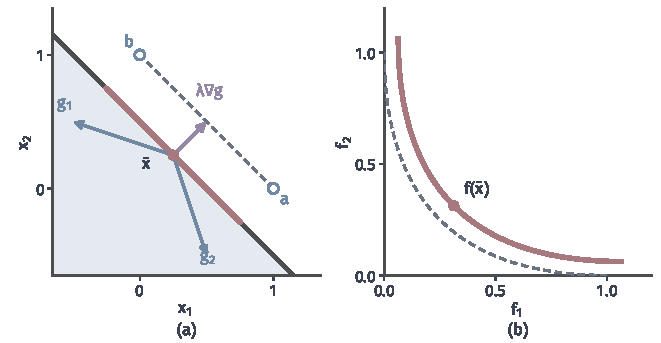
\includegraphics[width=112mm]{figures/05-optimization/07-multiple-criteria-and-nested-optimization/matplotlib/moo-feasible-pareto/figure.pdf}
  \caption{加上半平面约束$x_1+x_2\leq1/2$后的例子。(a)深灰粗线是活动约束，红色线段是约束下的解集（式~\eqref{eq:moo-feasible-set}），虚线是原来的解集；在$\bar{\bm{x}}=(1/4,1/4)$处，$\bm{g}_1,\bm{g}_2$的中点被紫色的$\lambda\nabla g$抵消。(b)红色曲线是约束下的前沿，虚线是原前沿，红点是$\bm{f}(\bar{\bm{x}})=(5/16,5/16)$。}
  \label{fig:moo-feasible-pareto}
\end{BookInlineFigure}

端点$\theta=0,1$的权重有零，但此时分别是$f_2$、$f_1$在可行集上的唯一最小点，由定理~\ref{thm:moo-weighted}的第~3条仍是Pareto最优点。这说明定理~\ref{thm:moo-kkt-sufficient}中“全正”只是充分条件，端点要单独检查。
